\documentclass[9pt, compress, xcolor=table]{beamer}


\usetheme{m}

\usepackage{amsmath,amssymb,amsthm}
\usepackage{latexsym}
\usepackage{booktabs}
\usepackage[scale=2]{ccicons}
\usepackage{minted}
% \usepackage[utf8]{inputenc}
% \usepackage[T2A]{fontenc}
% \usepackage[english, russian]{babel}
%%% For accessing system, OTF and TTF fonts
%%% (would have been loaded by polylossia anyway)
\usepackage{fontspec}
%%% For language switching -- like babel, but for xelatex
\usepackage{polyglossia}
%\setmainfont{PT Sans}  вообще шрифты определяются в теме бимера
\setmainlanguage{russian}
\setotherlanguages{english} %% or other languages

\usepackage{graphicx}
\usepackage{xcolor}
\usepackage{euscript}
% \DeclareMathOperator{\arctg}{arctg}
\usepackage{tabu} % https://ru.sharelatex.com/learn/Tables
\DeclareGraphicsExtensions{.pdf,.jpg,.png}
\graphicspath{{../images/}{./images/}}

\colorlet{Mycolor1}{green!50!blue!50!}
\DeclareMathOperator{\Ima}{Im}
\usemintedstyle{trac}

\title{Физические принципы микроскопии сверхвысокого разрешения}
\subtitle{осенний семестр, 2018}
\author{ассистент, к.ф.-м.н. Шутова О.А.}
\institute{МГУ им. М.В. Ломоносова, физический факультет}

\begin{document}

\maketitle

\plain{}{Лекция 12. Пространственная модуляция поля}

\begin{frame}{Основа метода}

{\small Метод SIM основан на пространственной модуляции поля вдоль оптической оси (эта возможность была осознана и реализована еще 1963 году), а также, и в настоящее время в первую очередь, в поперечной оптической оси плоскости, т.е. в плоскости объекта (1990 г.). Это достигается, в простейшем случае, посредством проецирования дифракционных решеток на плоскость объекта. Или созданием в области объекта интерферeнционной картины.

Следующим шагом стало привлечение нелинейного эффекта насыщения флуоресценции.

Возможность повышения разрешения является следствием свойств Фурье-преобразования. В качестве простой аналогии можно рассмотреть эффект Муара. Вспомним, как занавеска, изготовленная из волокна с характерным диаметром волокна, при наложении сама на себя дает локальный эффект прозрачности.}

\begin{center}
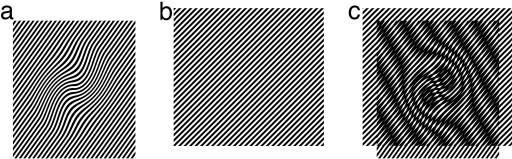
\includegraphics[width=0.8\textwidth]{moire_2}
\end{center}

\end{frame}

\begin{frame}{Свертка Фурье-компонент}
\begin{center}
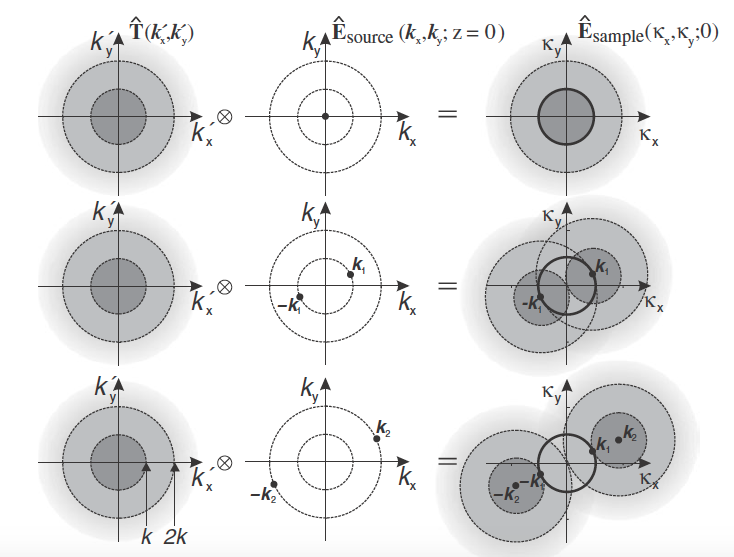
\includegraphics[width=0.7\textwidth]{ffm16}

\begin{equation*}
I(x,y) = I_0
(1+\cos [u x+\Delta)]
\end{equation*}
\begin{equation*}
F(x,y)=S(x,y) I(x,y)
\end{equation*}
\begin{equation*}
F(k_x,k_y)=\sqrt{2\pi} S(k_x,k_y)+\sqrt{\frac{\pi}{2}}\exp(-\imath \Delta)S(k_x-u,k_y)+\sqrt{\frac{\pi}{2}}\exp(\imath \Delta)S(k_x+u,k_y)
\end{equation*}

\end{center}
\end{frame}
\begin{frame}{Реконструкция изображения}

У нас есть три неизвестные величины:  $S(k_x,k_y)$, $S(k_x-u,k_y)$ и $S(k_x+u,k_y)$. Для их определения возмем три разные $\Delta$: $\Delta=0$, $\Delta = \frac{2\pi}{3}$ и $\Delta = \frac{4\pi}{3}$, решим систему из трех уравнений для $F(k_x,k_y)$ и тогда проведем обратное Фурье-преобразование

\begin{center}
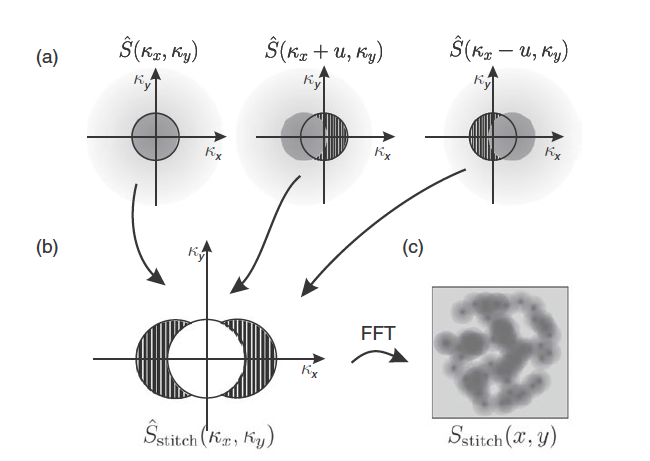
\includegraphics[width=0.8\textwidth]{ffm17}
\end{center}
\end{frame}

\begin{frame}{Численное моделирование}
    \begin{center}
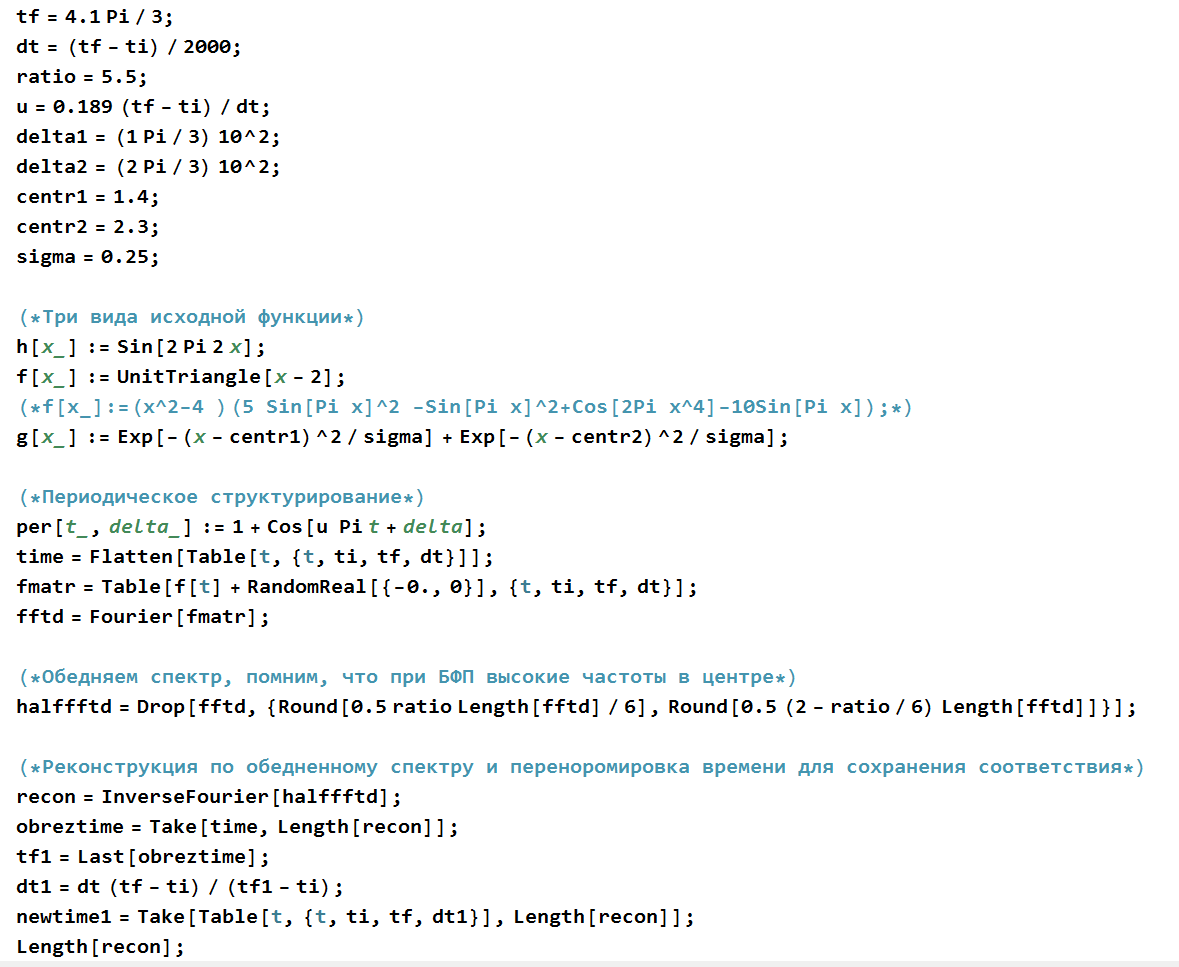
\includegraphics[width=0.95\textwidth]{prog1}
\end{center}
\end{frame}


\begin{frame}{Численное моделирование}
    \begin{center}
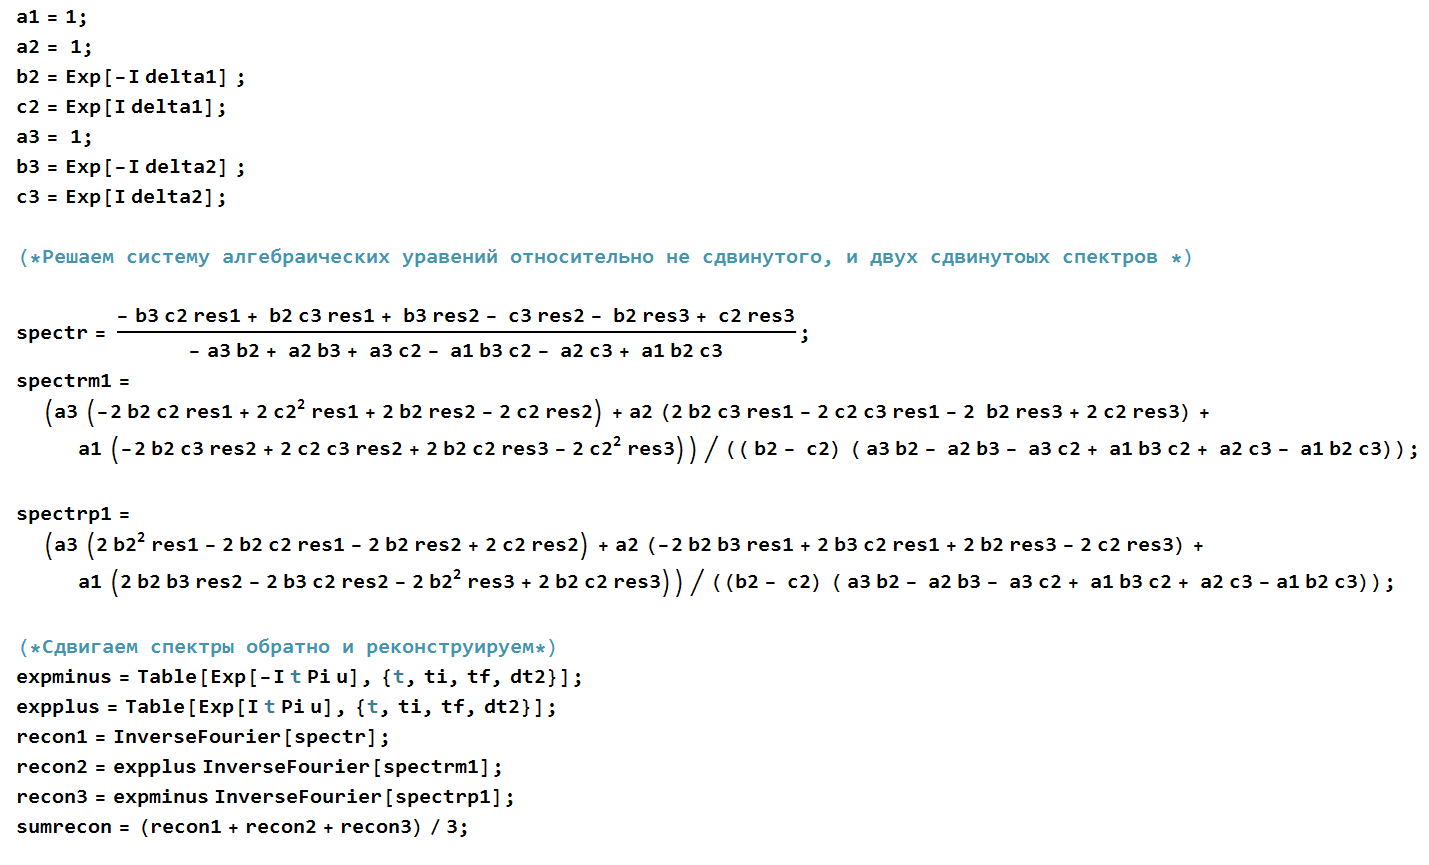
\includegraphics[width=\textwidth]{prog2}
\end{center}
\end{frame}


\begin{frame}{Численное моделирование}
\begin{columns}[c]
\column{6.5cm}
\begin{center}
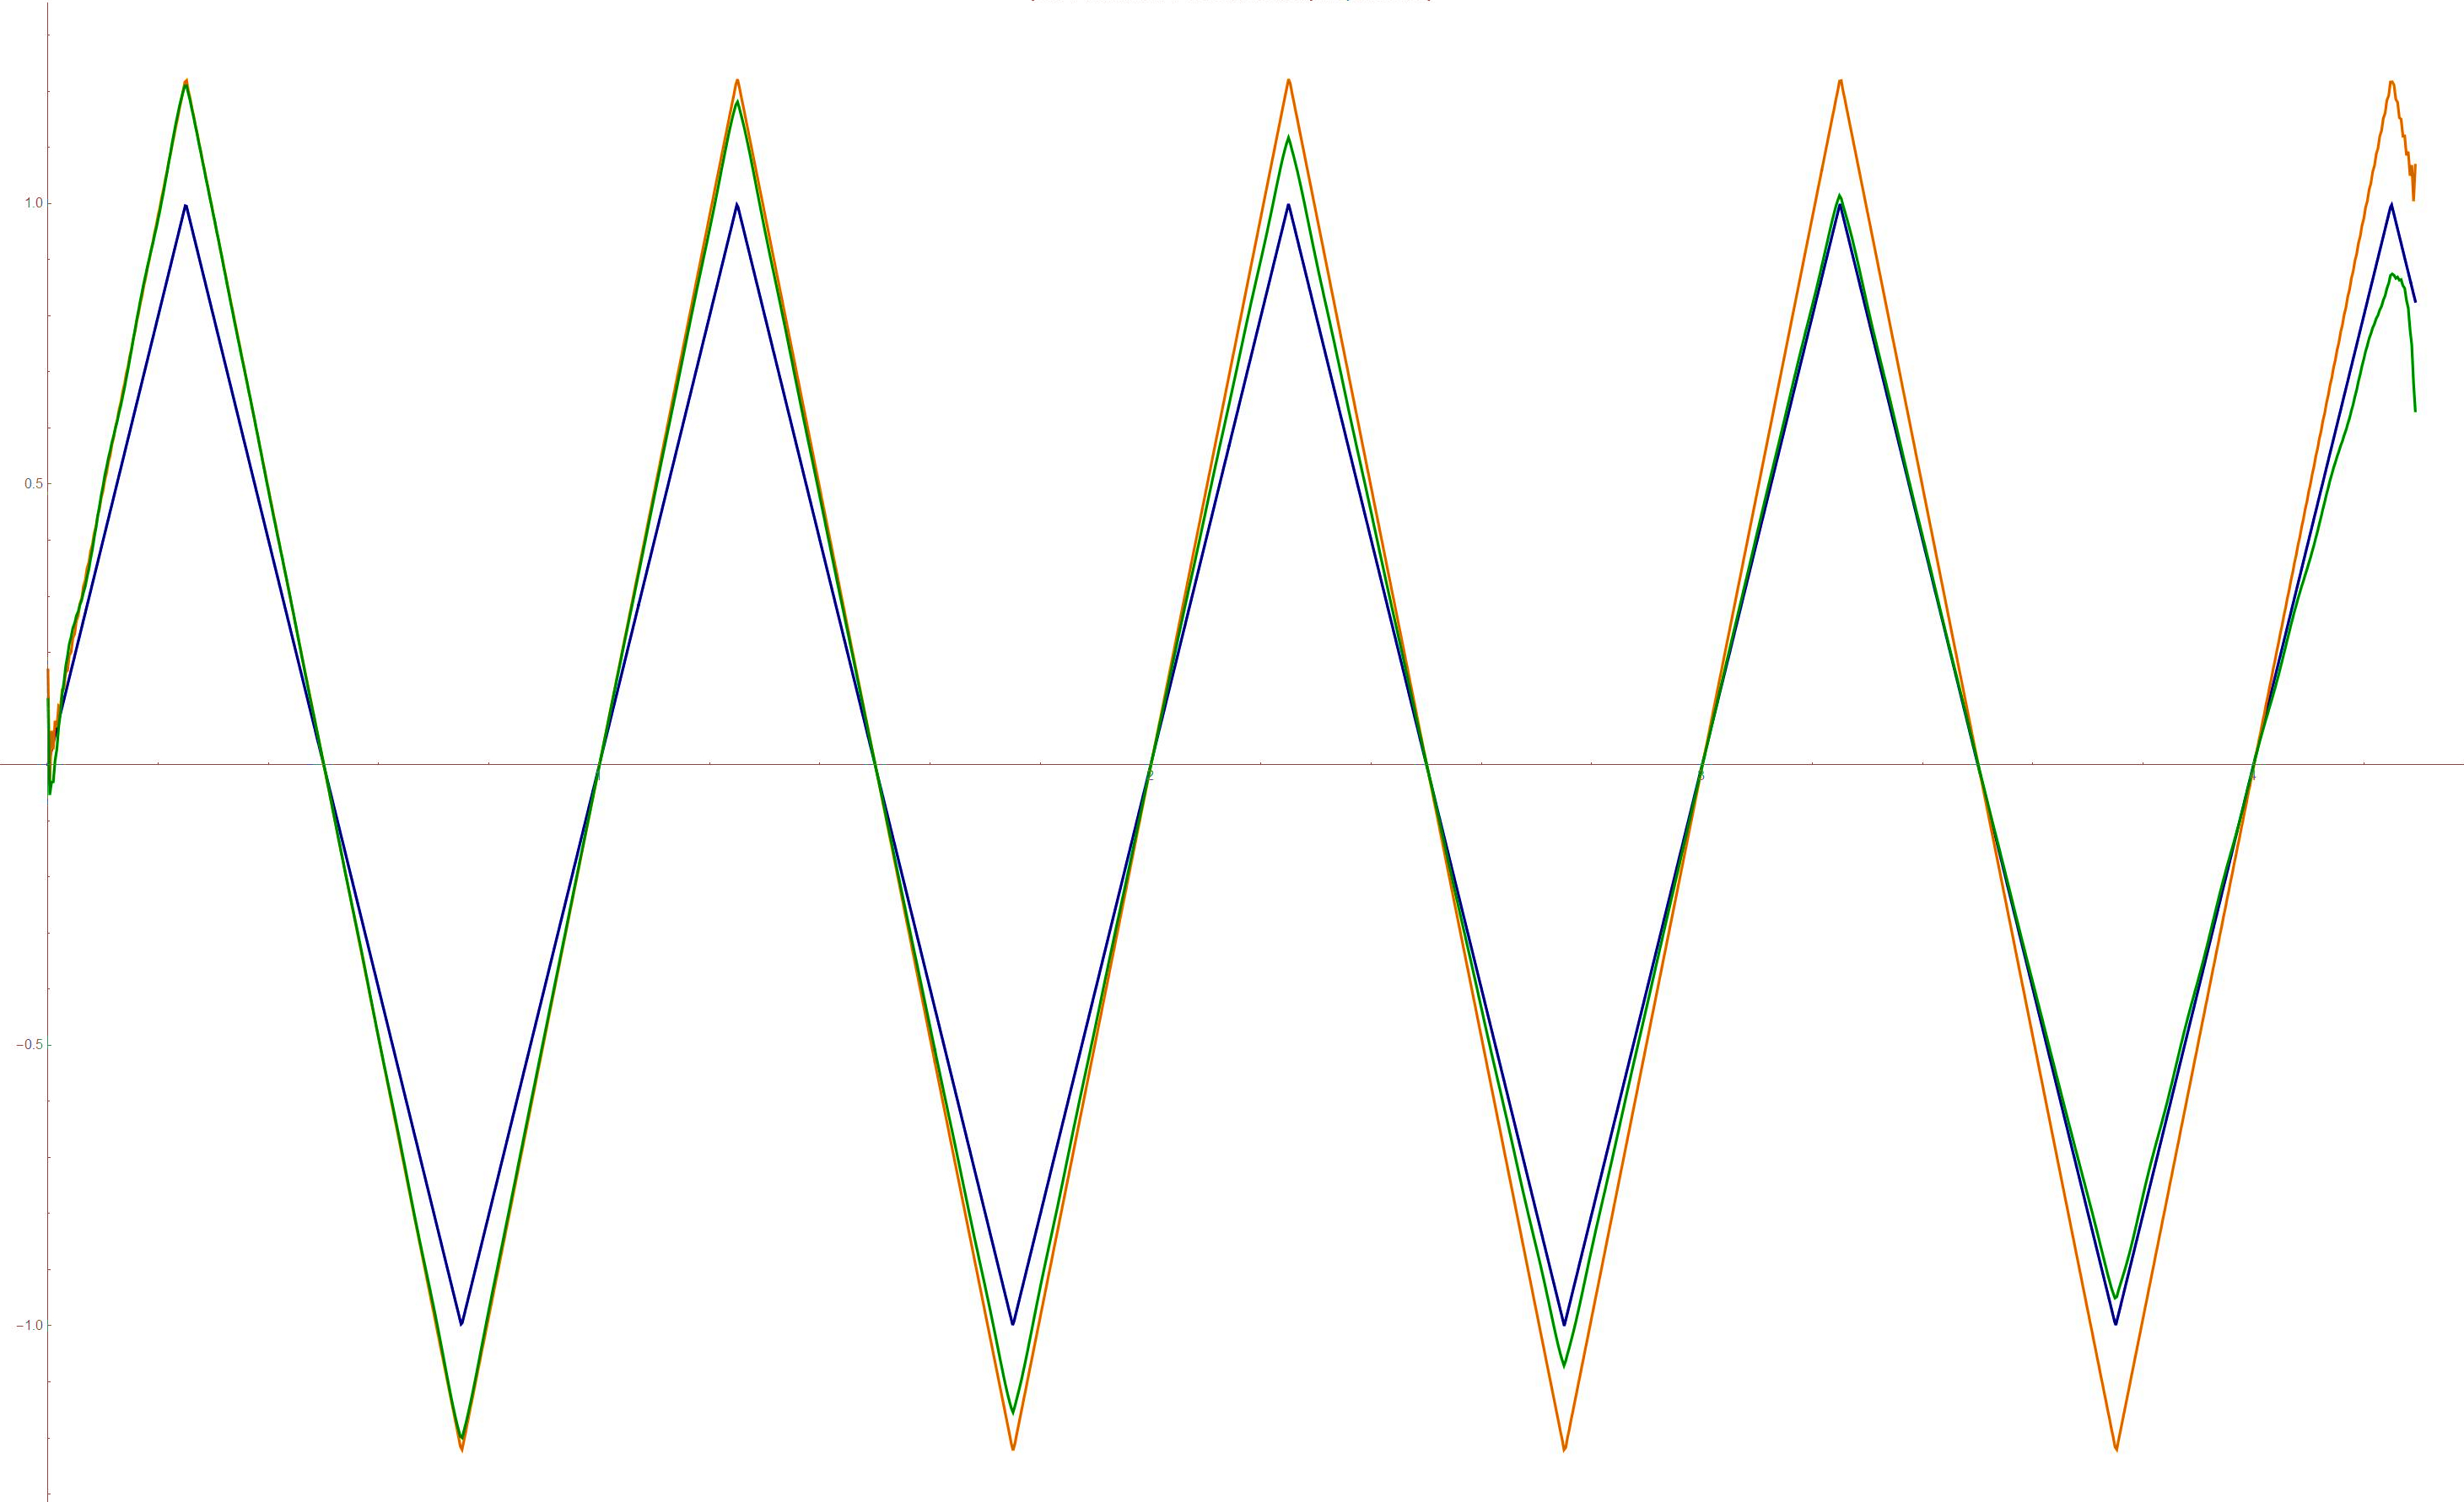
\includegraphics[width=0.9\textwidth]{triangle1.jpg}



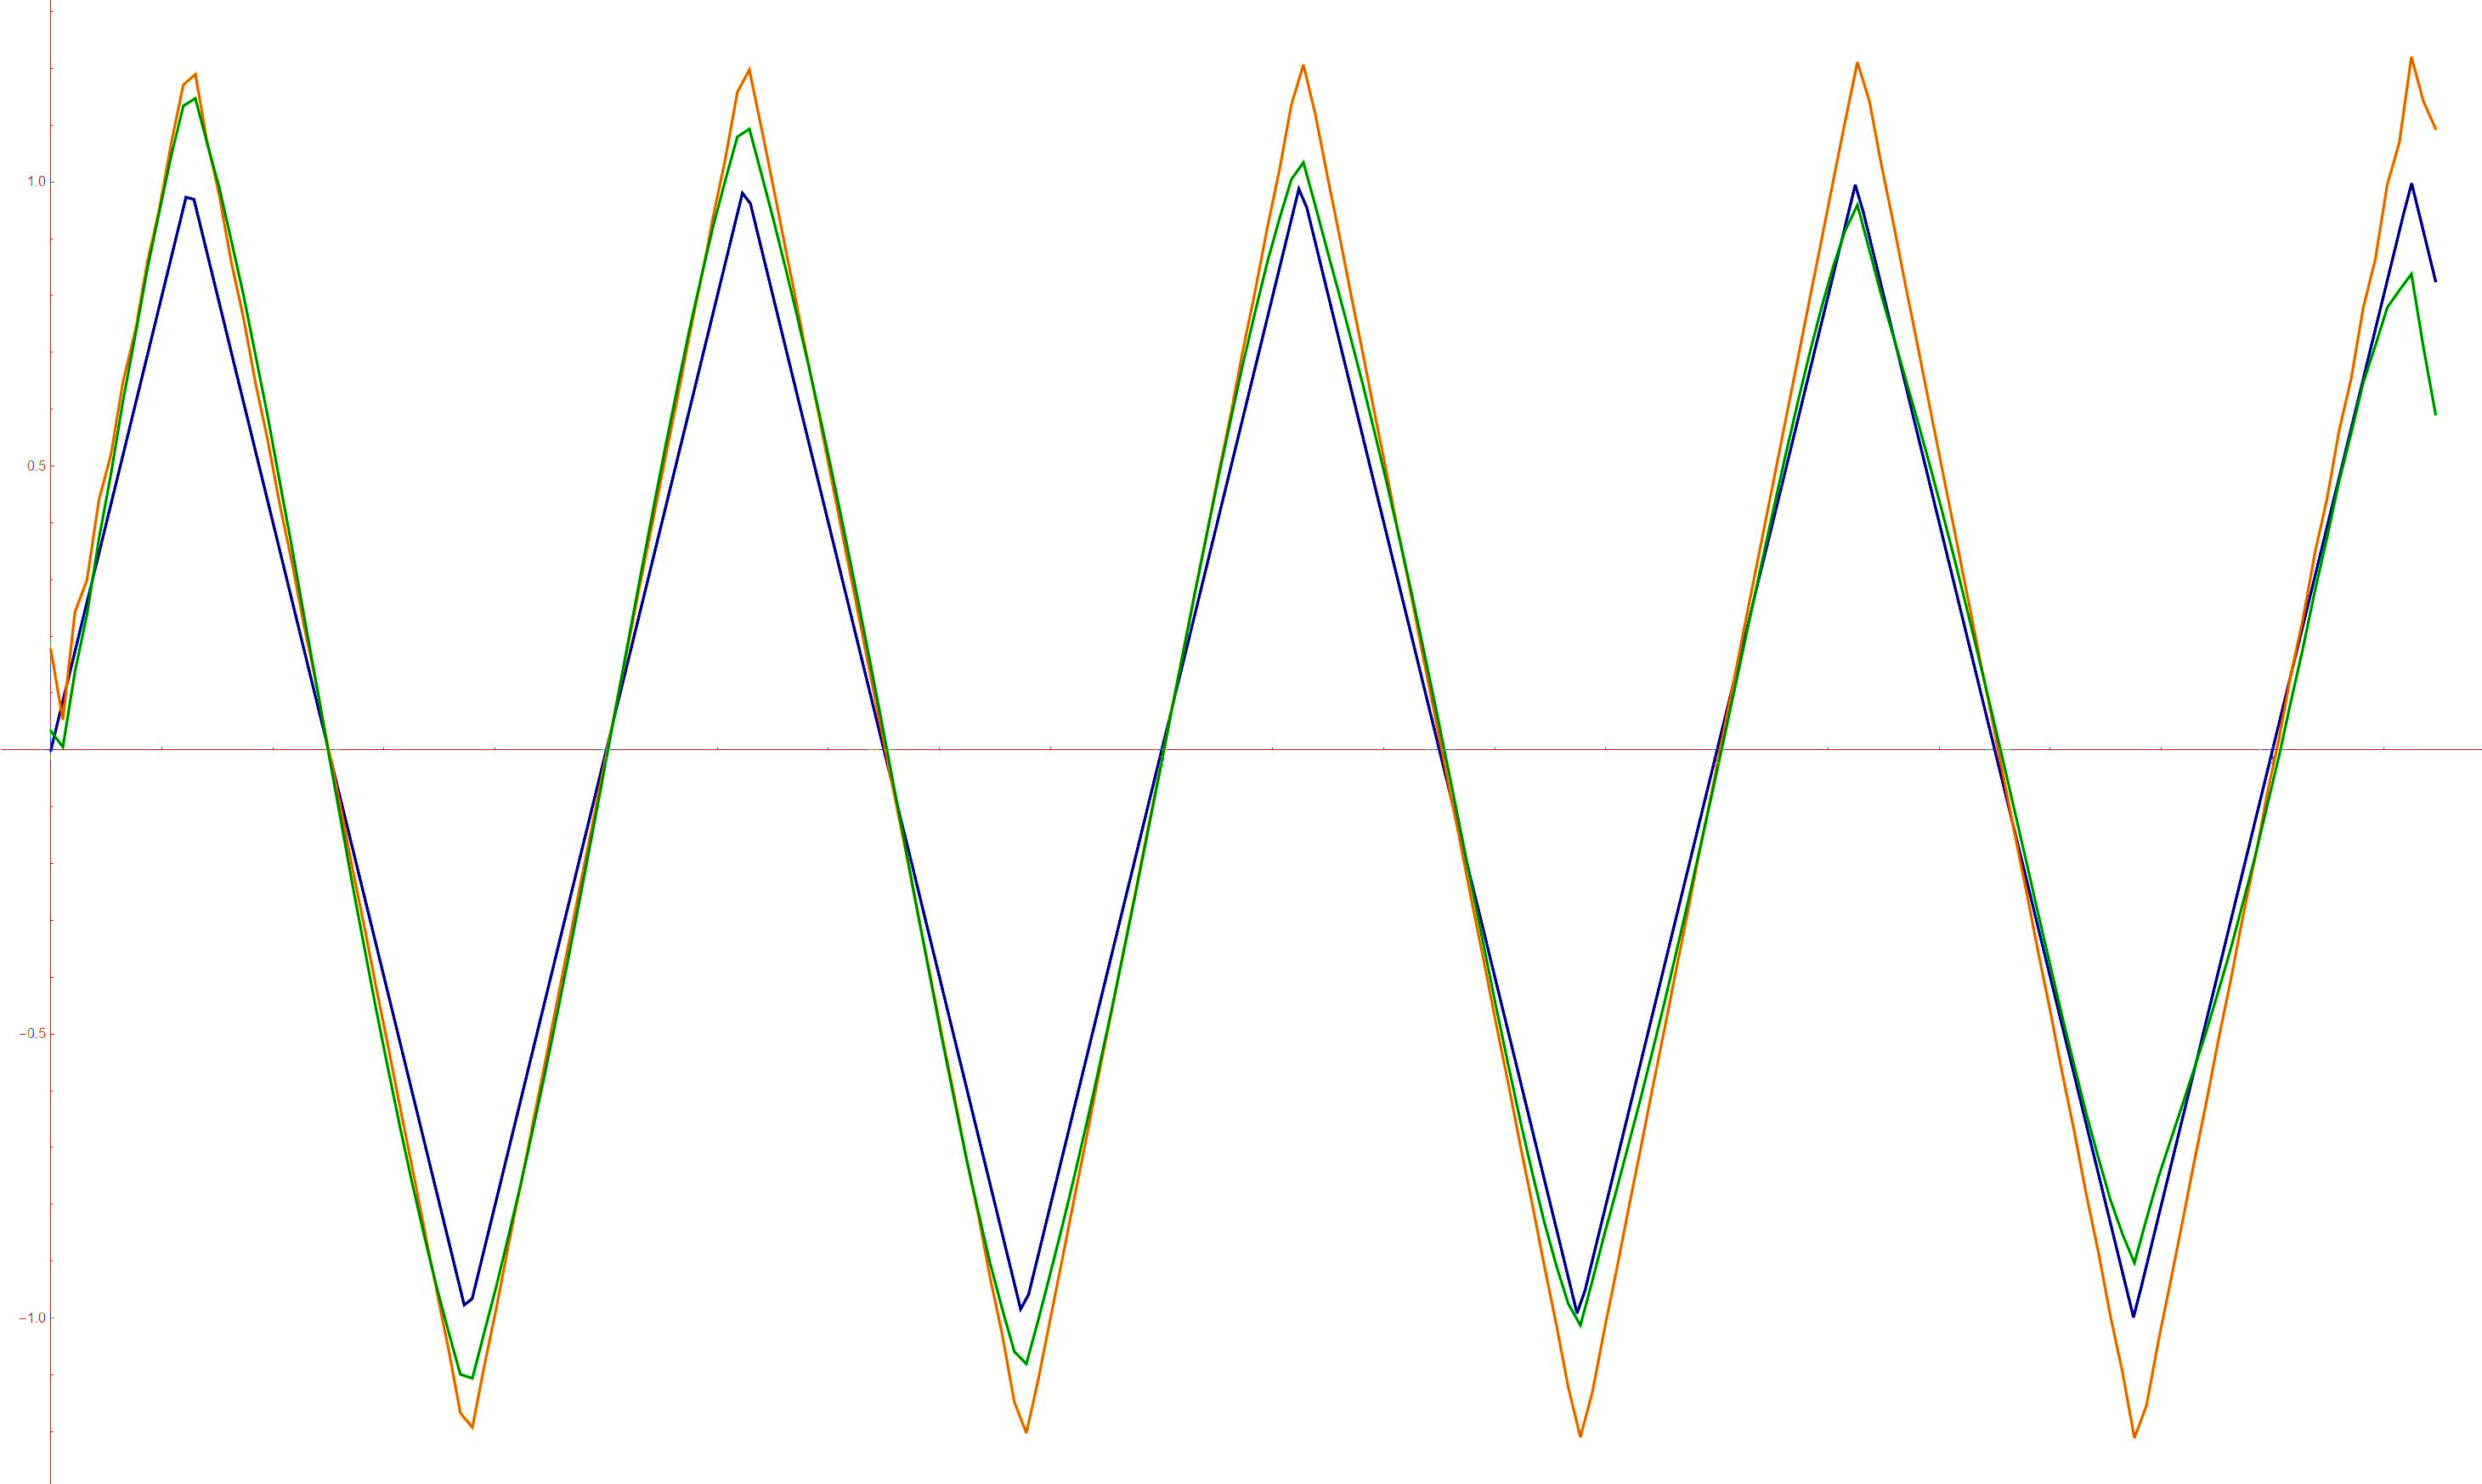
\includegraphics[width=0.9\textwidth]{triangle2.jpg}
\end{center}
\column{6.5cm}
\begin{center}
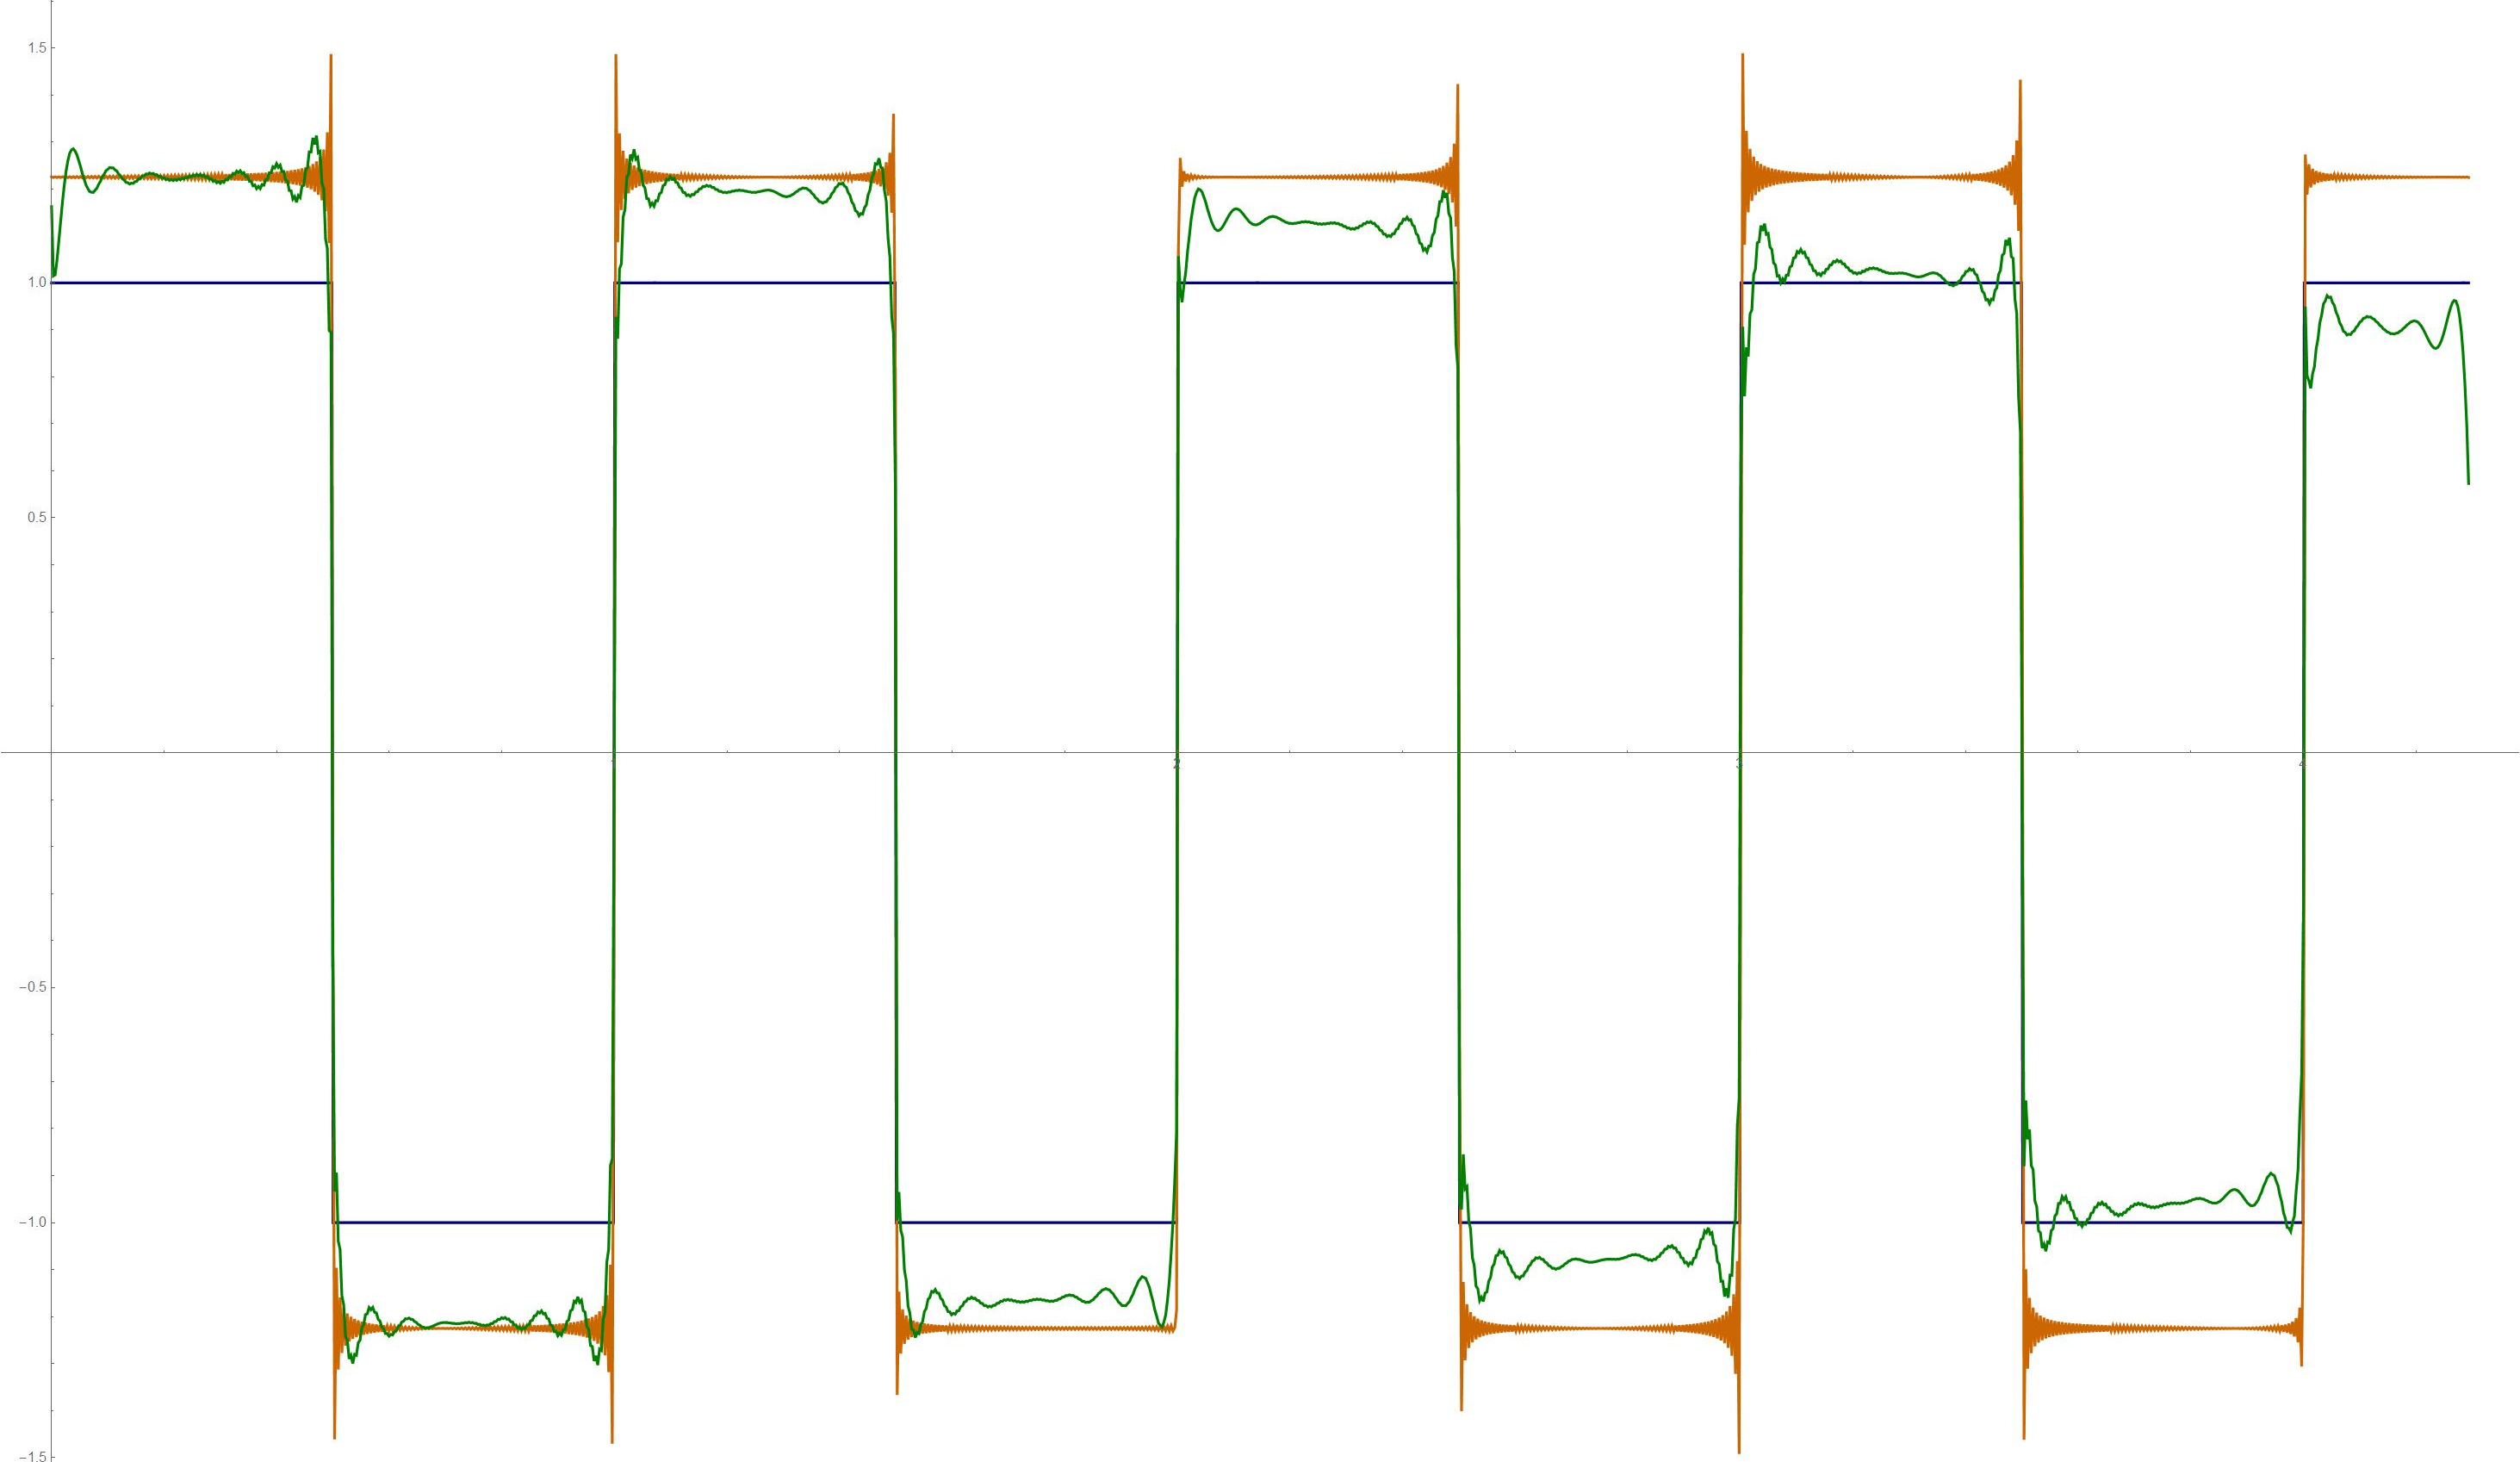
\includegraphics[width=0.9\textwidth]{square1.jpg}
\end{center}

\underline{Параметры:}
\begin{itemize}
    \item Частота обрезки задается длиной волны возбуждающего излучения и показателем преломления среды
    \item Величина сдвига определяется свойствами структурирования подсветки (периодом решетки, периодом стоячей волны и  т.д.)
    \item Частота Найквиста при дискретизации выбирается с учетом двух первых параметров 
\end{itemize}
\end{columns}
\end{frame}


\begin{frame}{Схема эксперимента продольного SIM}
\begin{columns}[c]
\column{7cm}
\begin{center}
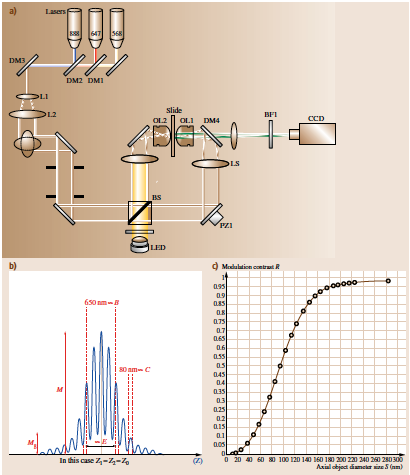
\includegraphics[width=0.85\textwidth]{ffm04}

{\small Такая микроскопия иногда называется микроскопией на стоячей волне}
\end{center}
\column{5.5cm}
\begin{center}
\textbf{ Кристоф Кремер (C. Cremer)}
 
 Если ввести такой параметр как контраст модуляции $R=\frac{M_G}{M}$, то проводя эксперимент с объектами известного диаметра, можно произвести калибровку такого микроскопа, получая зависимость продольного размера объекта от R.
 \begin{multline*}
 I(z)=\\=(M-M_G) sinc^2\left(\frac{z-z_1}{B}\right)*\cos[\frac{z-z_0}{C}]+\\+M_G sinc^2\left(\frac{z-z_2}{E}\right)+L
 \end{multline*}
 
 При этом константы $A,B,C,D,E$ явлюятся функциями $\lambda_{exc}$. То есть если $\lambda_{exc}$ не менять, R является функцииией размера объекта.
 
\end{center}
\end{columns}
\end{frame}

\begin{frame}{Схема эксперимента поперечного SIM на дифрак. решетке}
\begin{center}
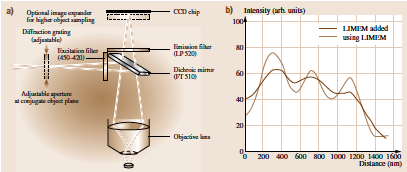
\includegraphics[width=\textwidth]{ffm05}
\end{center}

{\small Эксперимент по визуализации кварцевых шариков диаметром 416 нм, соединенных в "бусы". 

В таком подходе разрешающая способность не может быть увеличена более, чем в два раза.

См. книгу: Handbook of Lasers and Optics (Springer) Гл. 20. Cremer C. Optics Far beyond Diffraction Limit. 2012.}
\end{frame}

\begin{frame}{Схема эксперимента поперечного SIM на интерф. картинке}

Однако и в плоскости образца возможно создание интерференционного распределения поля, характеризующегося пространственной периодичностью. Для этого используются два или три поля.

\begin{center}
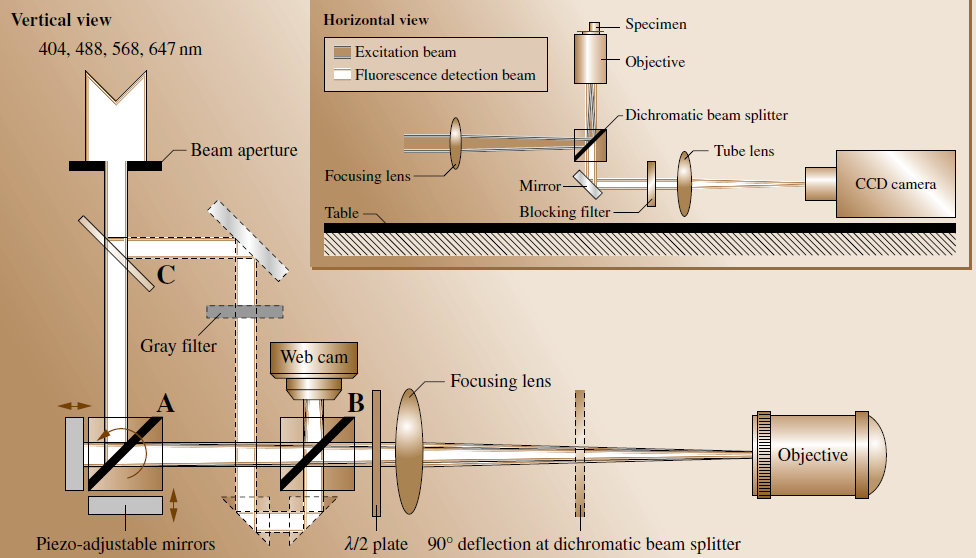
\includegraphics[width=0.9\textwidth]{sim23}
\end{center}
\end{frame}

\begin{frame}{Общее рассмотрение вопроса}
{\small Пусть распределение плотности флуоресцентных молекул $\rho$, структурирование поля $I$, а ФРТ оптической системы $PSF$. Тогда изображение:}
\begin{equation*}
g=PSF\otimes(\rho*I)
\end{equation*}
{\small Введем также оптическую функцию пропускания системы (OTF), как связь фурье-образов (как мы знаем, она действует как фильтр нижних частот, обрезая все, что ниже порога Аббэ):}
\begin{equation*}
FT(g)=OTF* FT(\rho)
\end{equation*}
{\small Рассмотрим случай двух плоских волн, падающих под углом $\pm\alpha$ к оптической оси:}
\begin{equation*}
E=E_{-1}\exp (-\imath[k(-\sin[\alpha x]+\cos[\alpha z])-\phi_1])+E_{+1}\exp (-\imath[k(\sin[\alpha x]+\cos[\alpha z])-\phi_2])
\end{equation*}

Если сигнал смотреть при разных $\phi_i=\phi_1-\phi_2$ (избегая точек, где фаза сингулярна), то можно для интенсивности на камере получим:
\begin{multline*}
I_{camera}(\phi_i) = \int_{\infty}^{\infty}dk_z
 FT[\rho(x,y,z) I(\phi_i)]*OTF=A+B_{+}\exp[+\imath \phi_i]+B_{-}\exp[-\imath \phi_i]+\\+C_{+}\exp[+2\imath \phi_i]+C_{+}\exp[-2\imath \phi_i]\end{multline*}

Следовательно необходимо измерить в пяти точках по фазе.

\end{frame}

\begin{frame}{Исследование ткани сетчатки глаза человека}

С помощью трехлучевой установки (488, 568 и 647 нм)
\begin{center}
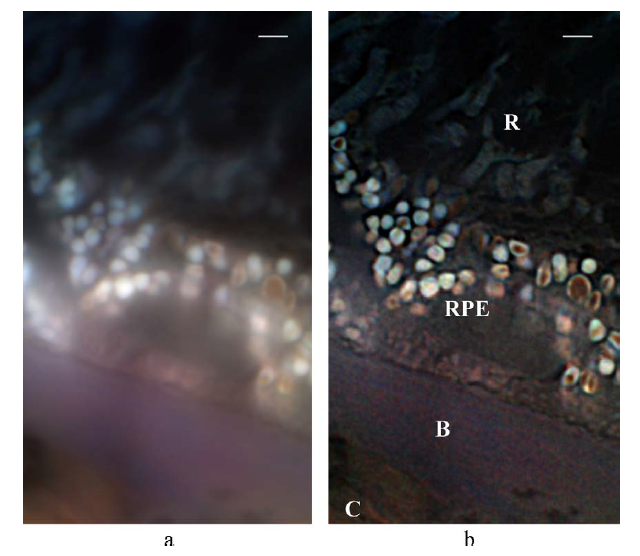
\includegraphics[width=0.75\textwidth]{sim11}
\end{center}
(масштабный отрезок 2 микрона)
\end{frame}

\begin{frame}{Исследование ткани сетчатки глаза человека}

RPE - пигментный эпителий сетчатки

R - видны концы клеток палочек 

B - мембрана Брача

\begin{center}
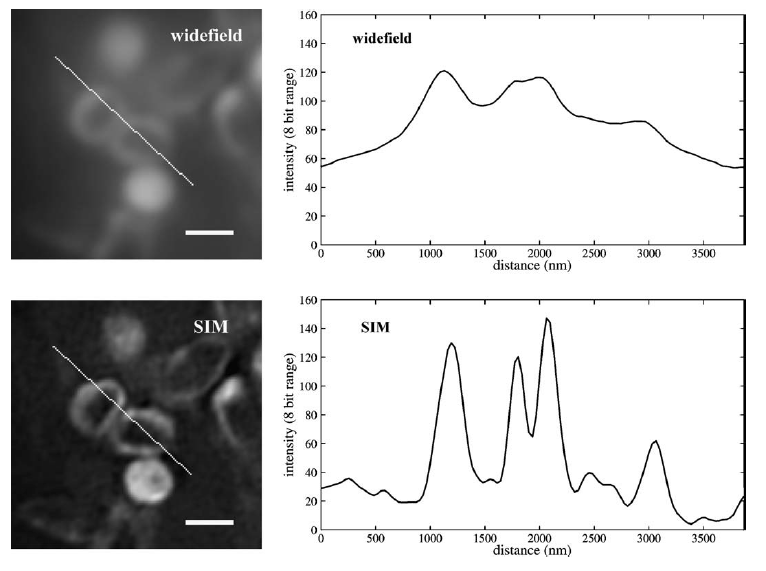
\includegraphics[width=0.8\textwidth]{sim12}
\end{center}

\end{frame}

\begin{frame}{Два вида гранул}

LF - липофусцин

MLF - меланолипофусцин

\begin{center}
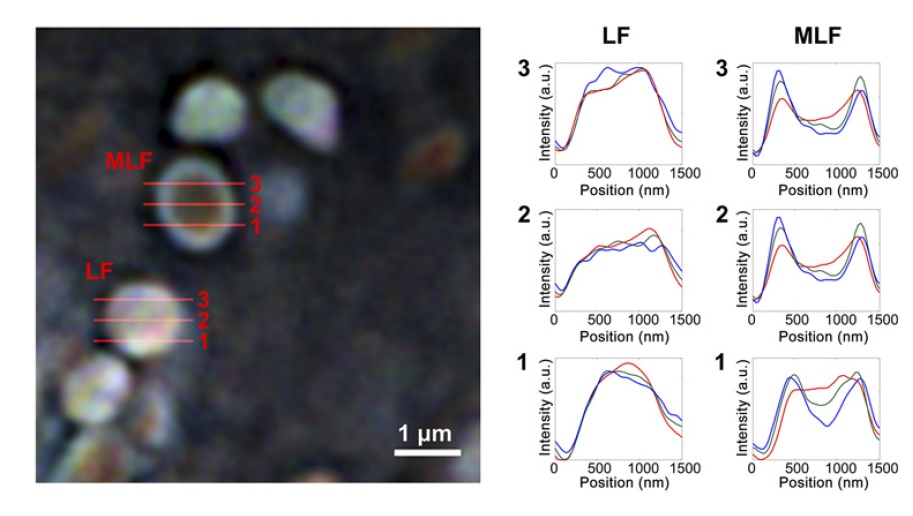
\includegraphics[width=0.8\textwidth]{nlsim14}
\end{center}

\end{frame}

\plain{}{Нелинейная микроскопия структурированной подсветки}

\begin{frame}{Высокие гармоники}

Для получения более высоких порядков нет другого способа, кроме введения нелинейности. Таким нелинейным процессом может послужить насыщение флуоресценции.
\begin{center}
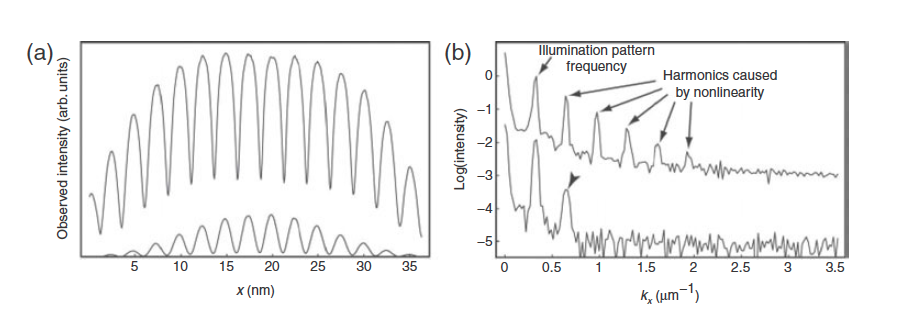
\includegraphics[width=0.9\textwidth]{ffm18}
\end{center}

\begin{equation*}
\boxed{Min[\Delta r_{||}]=\frac{\lambda}{2\pi (2+l)NA}}
\end{equation*}

где $l$ - максимально достижимый порядок нелинейности. Необходимо иметь ввиду, что и количество неизвестных соответственно возрастает, и сканировать фазу приходится с очень малым шагом.
\end{frame}

\begin{frame}{Насыщение флуоресценции}

В области насыщения скорость флуоресценции зависит от интенсивности нелинейно:

\begin{equation*}
R(I)=R_0\frac{I/I_S}{1+I/I_S}
\end{equation*}

\begin{center}
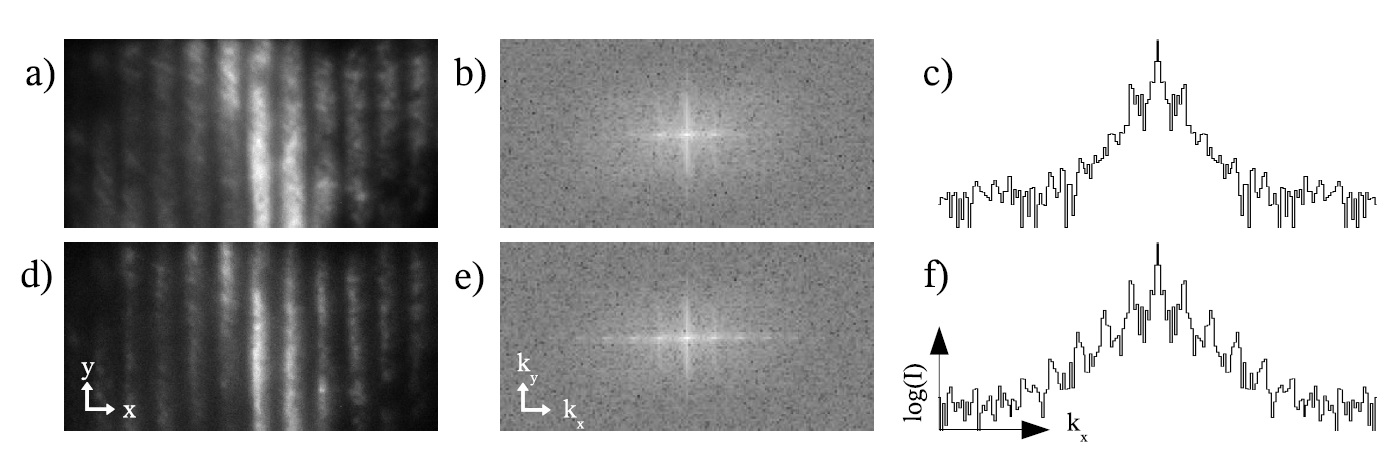
\includegraphics[width=0.9\textwidth]{nlsim13}
\end{center}

Изображение дифракционной решетки с периодом 1.8 микрон в области линейной флуоресценции (верхний ряд) и в области насыщения (нижний ряд, видим, что добавляются дополнительные гармоники).

R. Heintzmann et al. King's College London. 2013.


\end{frame}

\begin{frame}{Дронпа}
\begin{columns}[c]
\column{6.5cm}
\begin{center}
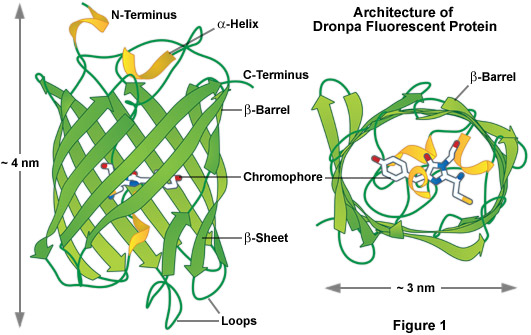
\includegraphics[width=0.9\textwidth]{nlsim5}

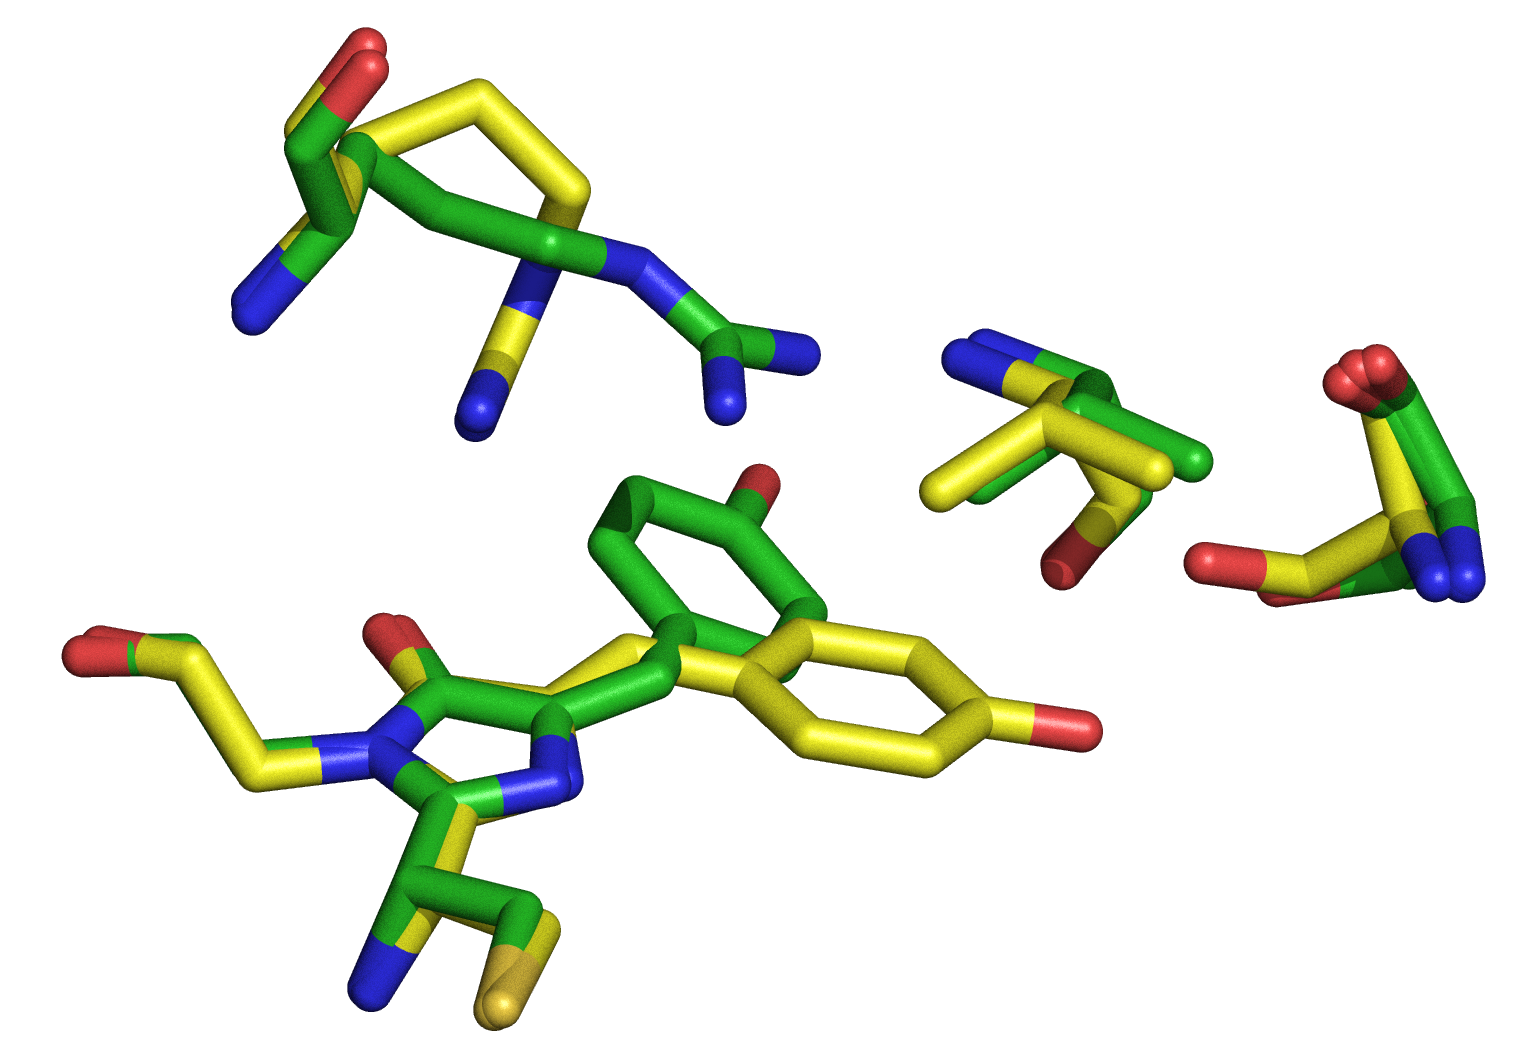
\includegraphics[width=0.8\textwidth]{nlsim4}
\end{center}
\column{6.5cm}
\begin{center}
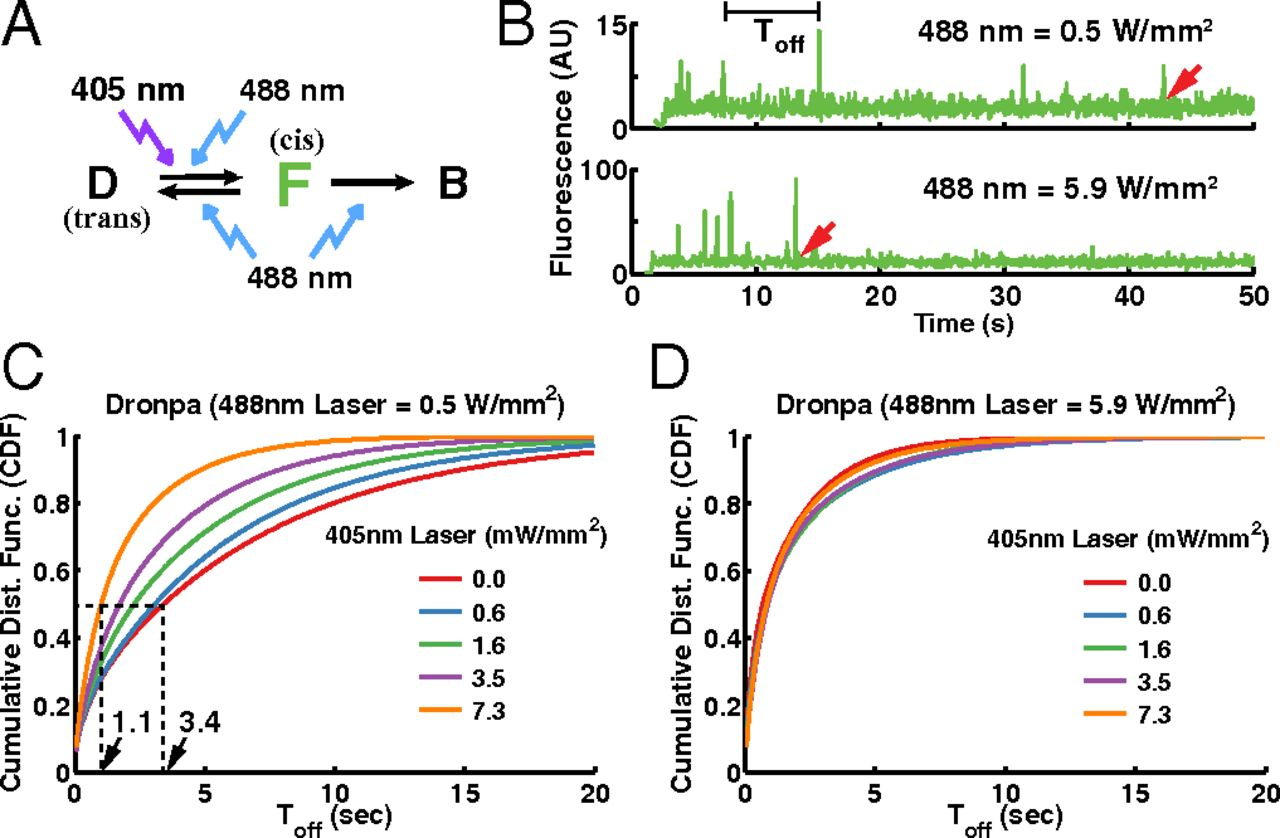
\includegraphics[width=0.9\textwidth]{nlsim6}
\end{center}

{\small Дронпа - фотопереключаемый белок. Важны два параметра: отношение интенсивности в состоянии "on" к интенсивности в состоянии "off" (этот параметр зависит от близости к насыщению), а также скорость фотообесцвечивания (60-70 проходов при интенсивности $5 \text{Вт/см}^2$).}

\end{columns}

\end{frame}

\begin{frame}{Нелинейная SIM}
\begin{center}

Работы М. Густавссона, Университет Калифорнии (M. Gustafsson, 2012)

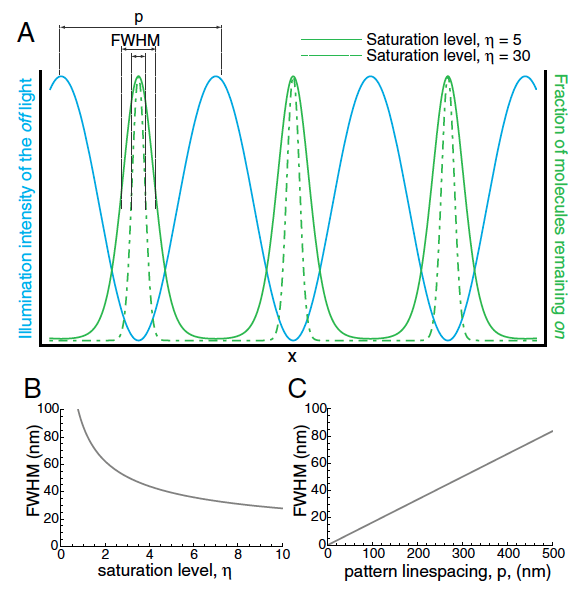
\includegraphics[width=0.7\textwidth]{nlsim7}
\end{center}
\end{frame}

\begin{frame}{Нелинейная SIM}
\begin{center}
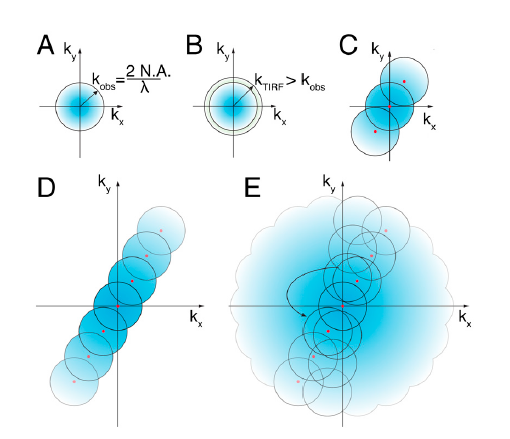
\includegraphics[width=0.8\textwidth]{nlsim8}
\end{center}
\end{frame}

\begin{frame}{Нелинейная SIM}
\begin{center}
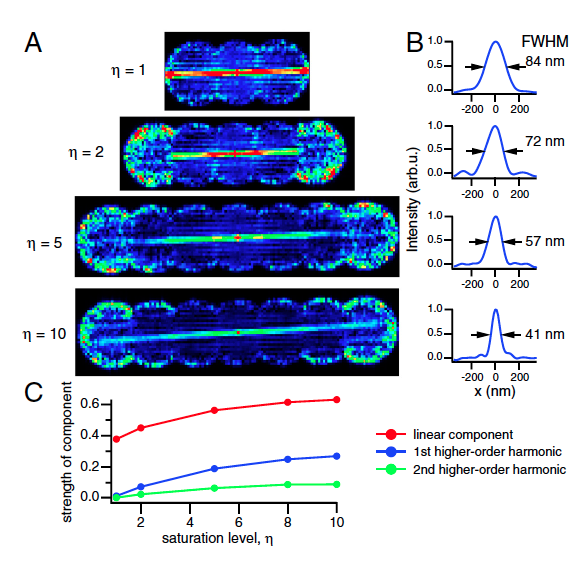
\includegraphics[width=0.8\textwidth]{nlsim9}
\end{center}
\end{frame}

\begin{frame}{Нелинейная SIM}
\begin{center}
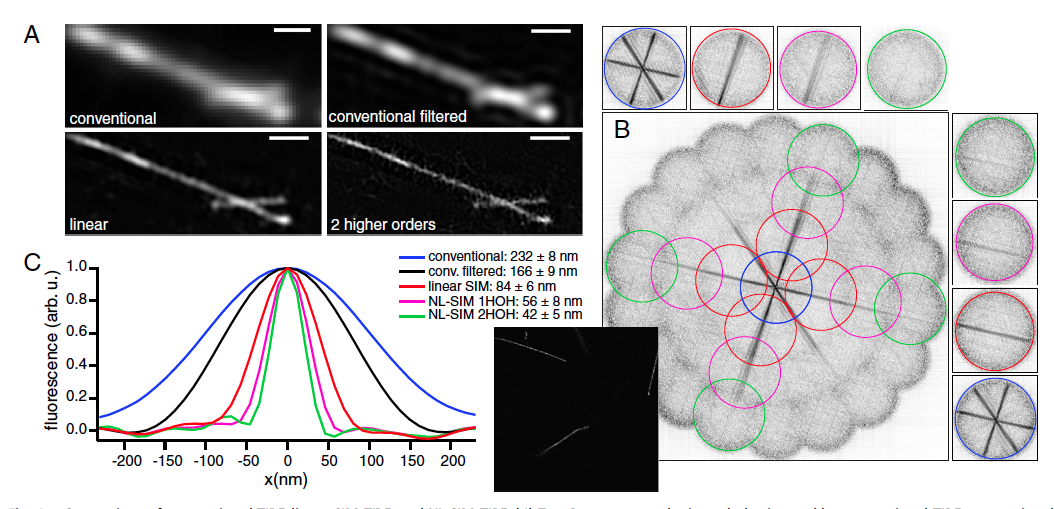
\includegraphics[width=0.9\textwidth]{nlsim10}
\end{center}
\end{frame}

\begin{frame}{Нелинейная SIM}
\begin{center}
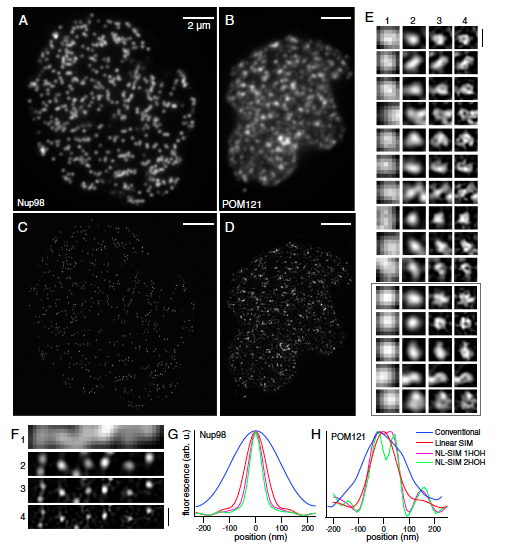
\includegraphics[width=0.6\textwidth]{nlsim11}
\end{center}
\end{frame}

\begin{frame}{Нелинейная SIM}
\begin{center}
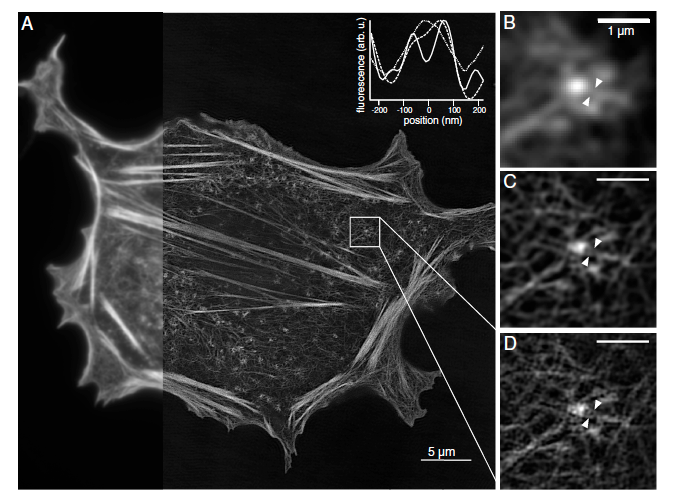
\includegraphics[width=0.9\textwidth]{nlsim12}
\end{center}
\end{frame}


\begin{frame}{Работа 2017 г.}
Chemical Reviews. 2017

Reiner Heitzmann, Thomas Huser.
\begin{center}
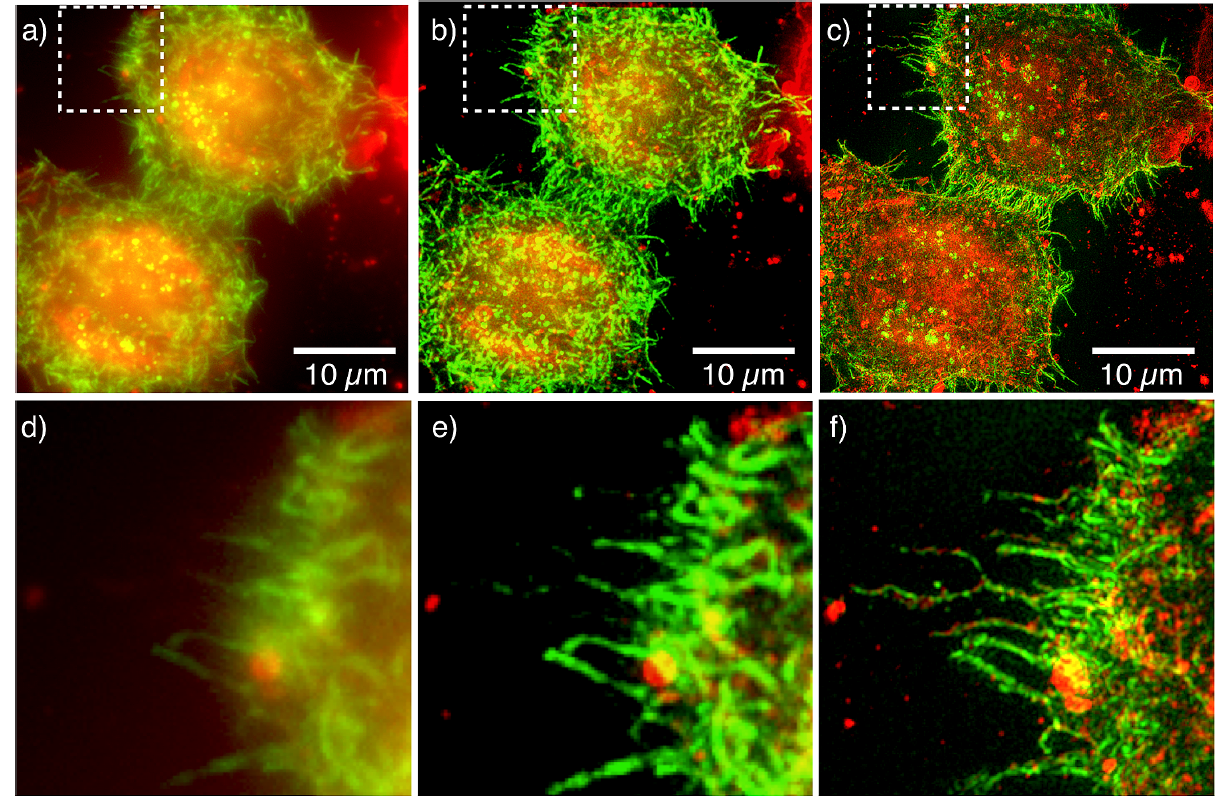
\includegraphics[width=0.9\textwidth]{sim_2017.png}

Микрофотографии клеток остеосаркомы (U2OS) по методу широкопольной флуоресцентной в  эписхеме (а), реконструкция
данных эпифлуоресценции (b) и 3D-SIM (c). Зеленый канал цвета кодирует трансмембранную субъединицу β-дистрогликан-eGFP, красный 
канал выделяет плазменную мембрану, окрашенную оранжевой клеткой CellMask. 

\end{center}
\end{frame}

\end{document}


\begin{frame}{}
\begin{columns}[c]
\column{6.5cm}
\begin{center}
\includegraphics[width=0.9\textwidth]{}
\end{center}
\column{6.5cm}
\begin{center}
\includegraphics[width=0.9\textwidth]{}
\end{center}
\end{columns}
\end{frame}

\begin{frame}{}
\begin{center}
\includegraphics[width=0.9\textwidth]{}
\end{center}
\end{frame}

Понятно, что такой сдвиг позволит получить лишь незначительное превышение дифракционного предела. Для лучшего эффекта необходимо включать нелинейности отклика.